\documentclass{article}

\usepackage{tabularx}
\usepackage[table]{xcolor}
\usepackage{hyperref}
\usepackage{cleveref}
\usepackage{tikz}
\usetikzlibrary{positioning, calc, shapes, arrows, fit}
\usepackage{circuitikz}
\usepackage{subcaption}
\usepackage[colorinlistoftodos]{todonotes}
\linespread{0.9}
\hypersetup{
    colorlinks = true,
    linkbordercolor = {black}
}
\begin{document}
\title{Lab 1 -- Measuring ``Parasitics'' of Passive Components with a VNA}
\author{
    Yifan Zhu\\
    Lab Partner: John Kustin
}
\maketitle

\begin{abstract}
    S-Parameters of passive components are measured using a Vector Network Analyzer (VNA), and more realistic circuit models containing parasitics are proposed.
    The proposed circuit models are simulated in LTSPice, and compared against the experimentally obtained results.
\end{abstract}

\section{Introduction}
Real life passive components are far from ideal.
All capacitors, inductors, and resistors have some parasitic capacitance, inductance, and resistance.
But how can we measure these parasitics?
How can we build good electric models of these real-world componenets?
To this end, we use Vector Network Analyzers (VNA) to measure the frequency response of these passive components, use our understanding of circuit elements to conjecture about good circuit models, and use LTSpice to verify that the circuit models match what we observe.

\section{Experimental Setup}
\begin{figure}[h]
    \centering
    \begin{subfigure}{.5\linewidth}
        \centering
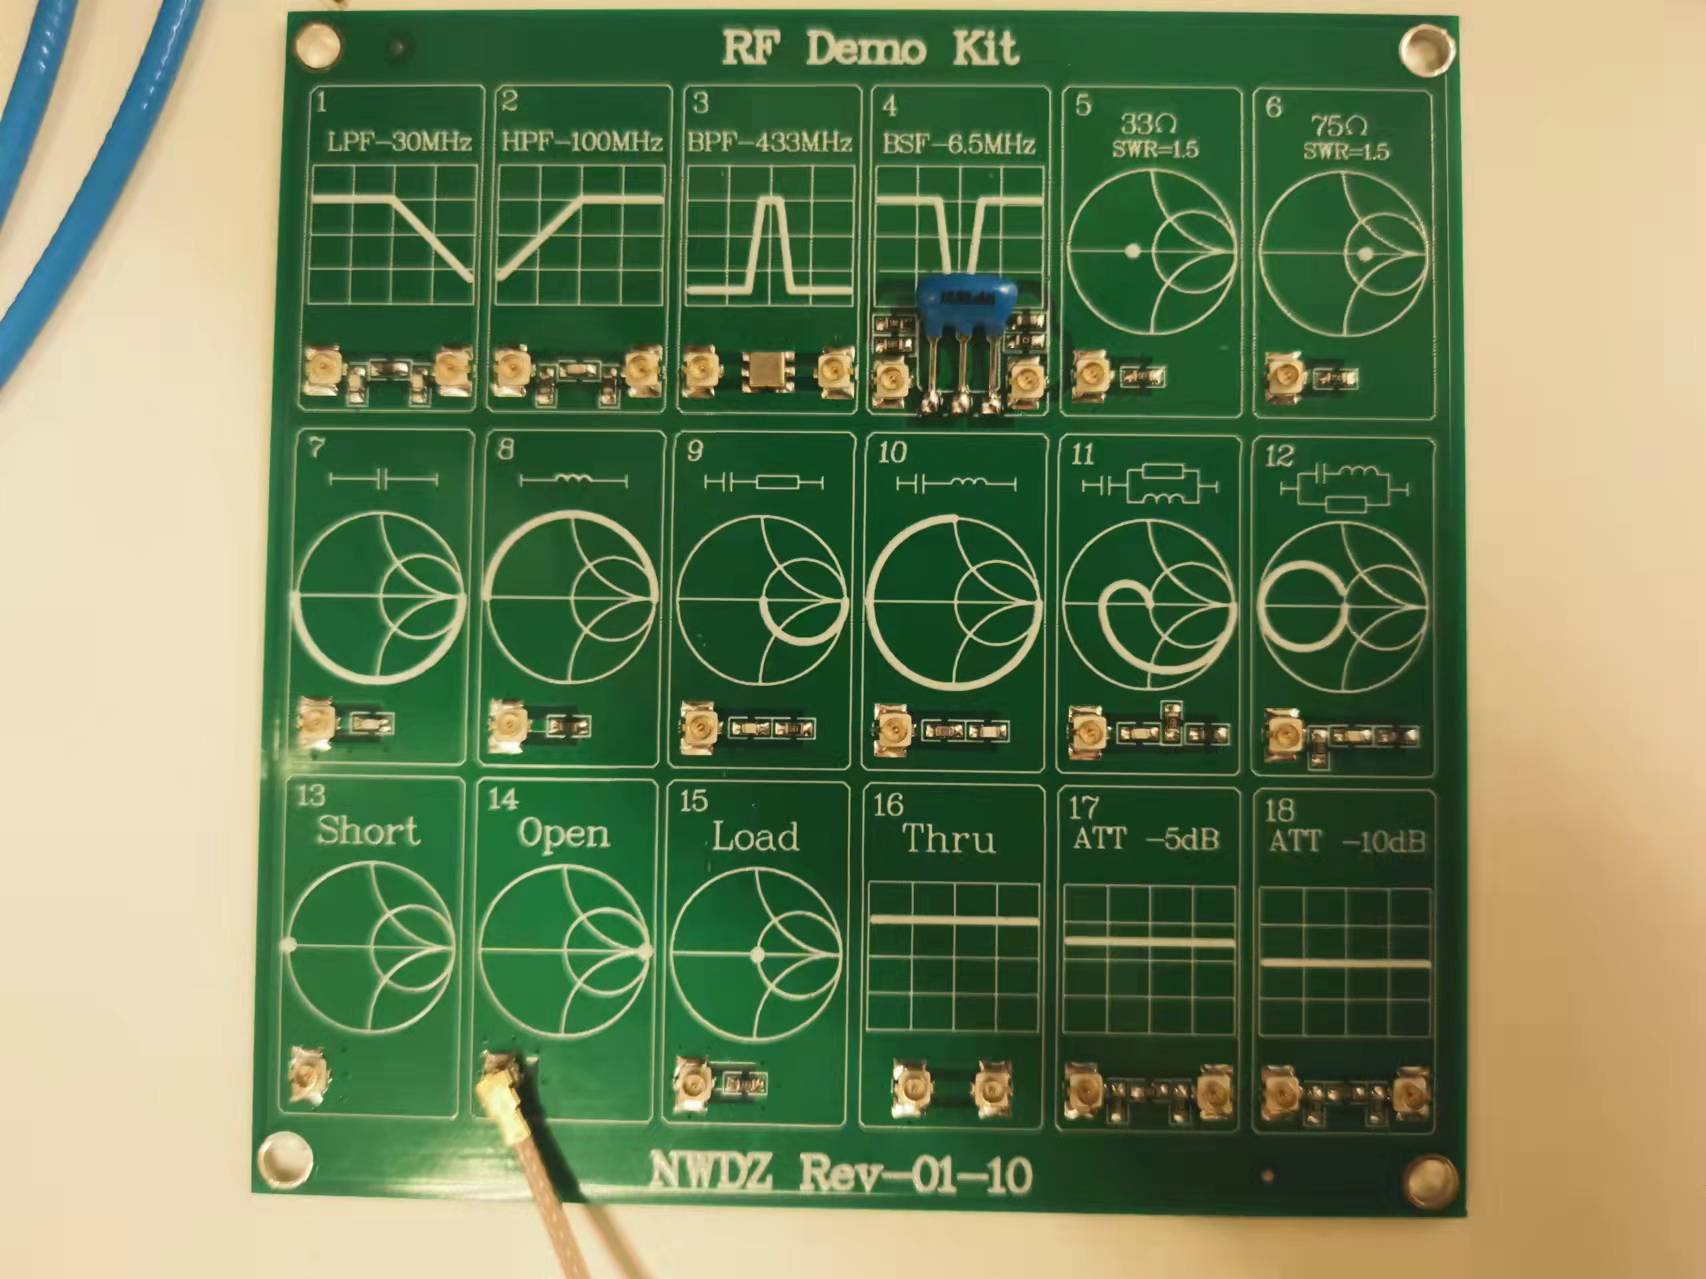
\includegraphics[width=.8\linewidth]{./pics/test_loads.jpg}
        \caption{Picture of RF Demo Kit NWDZ}
        \label{fig:test_loads}
    \end{subfigure}%
    \begin{subfigure}{.5\linewidth}
        \centering
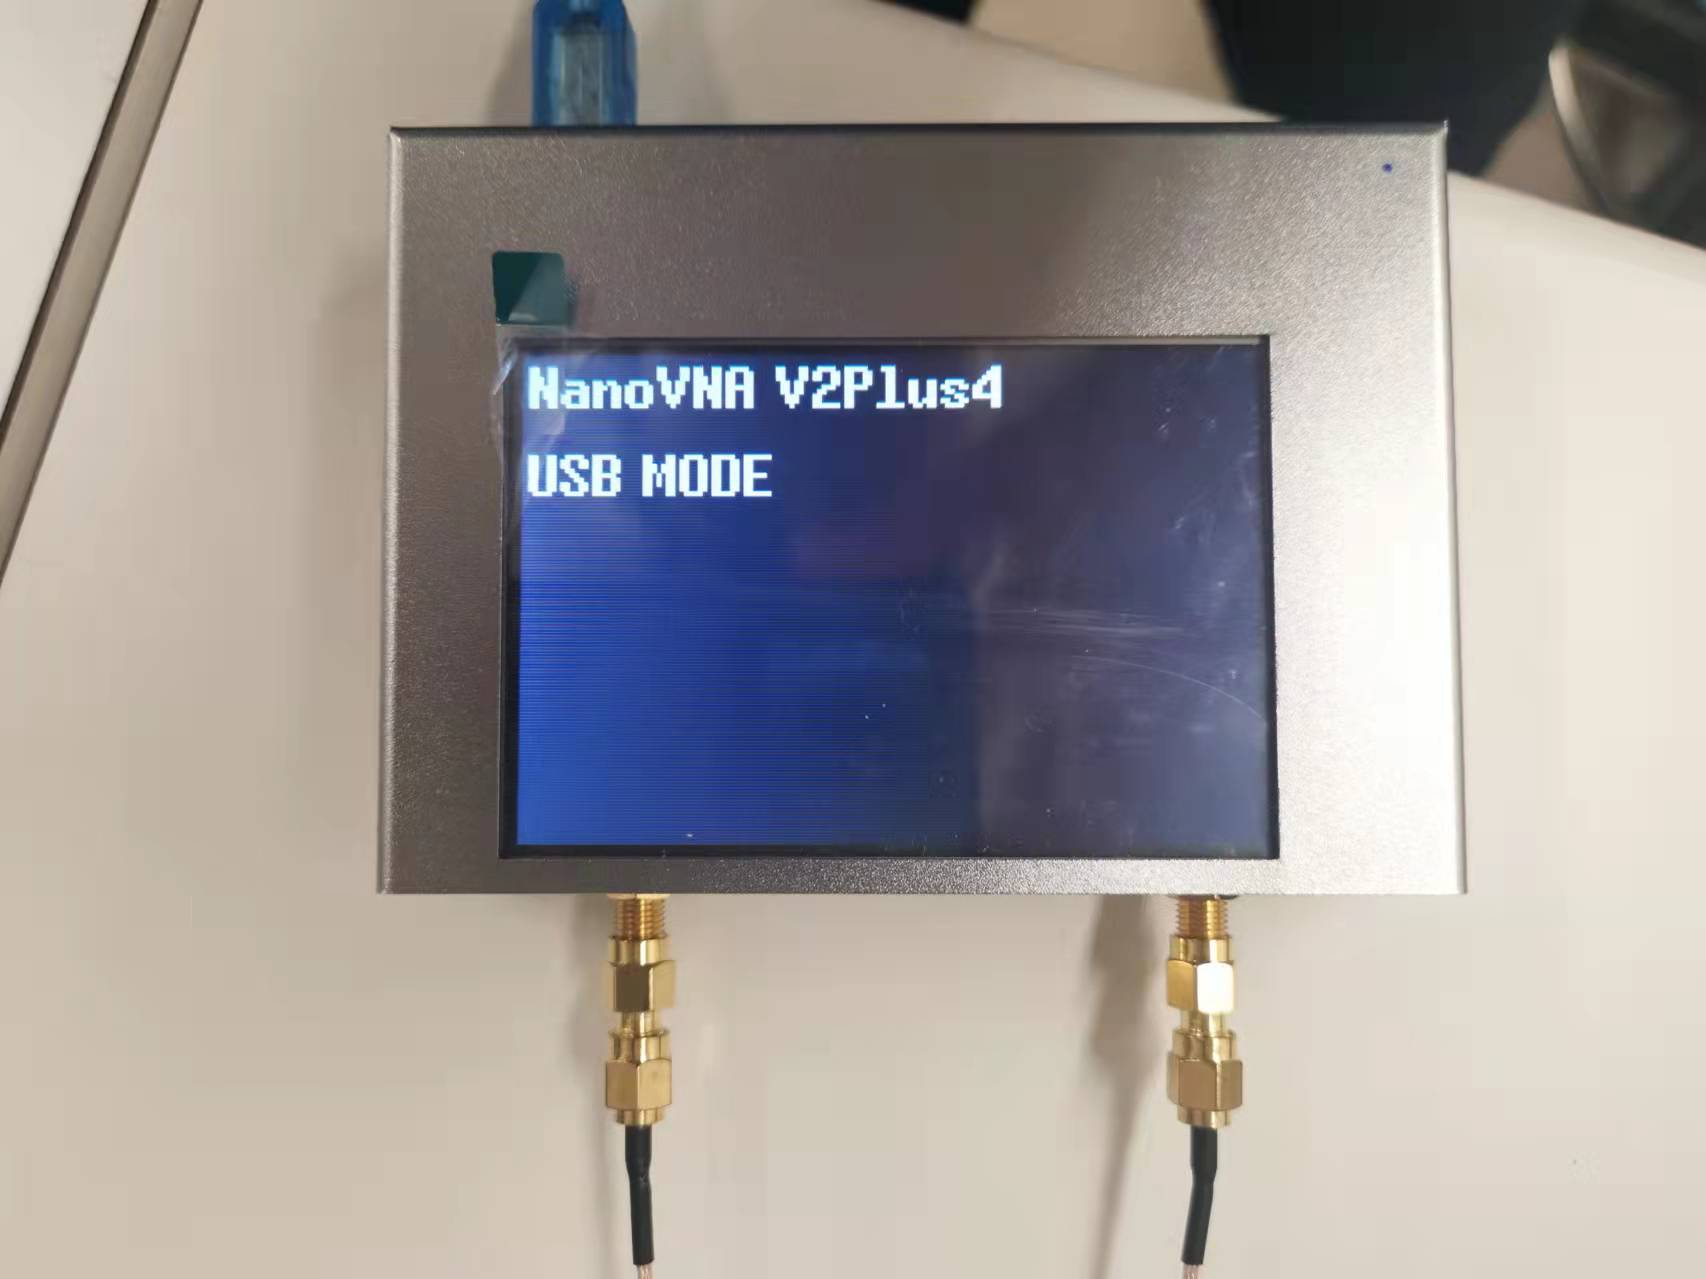
\includegraphics[width=.8\linewidth]{./pics/NanoVNA.jpg}
        \caption{Picture of NanoVNA}
        \label{fig:nanovna}
    \end{subfigure}
\caption{Picture of Tools used in Experiment}
\end{figure}

The passive componenets of interest are all surface mount components on the \emph{RF Demo Kit NWDZ Rev-01-10} (\Cref{fig:test_loads}), and
we use the NanoVNA (\Cref{fig:nanovna}) to perform the measurements.
Care is taken to calibrate the NanoVNA each time before use.

\section{Measurements and Results}

\subsection{Capacitor}
\begin{figure}[h]
    \centering
    \begin{subfigure}{0.5\linewidth}
        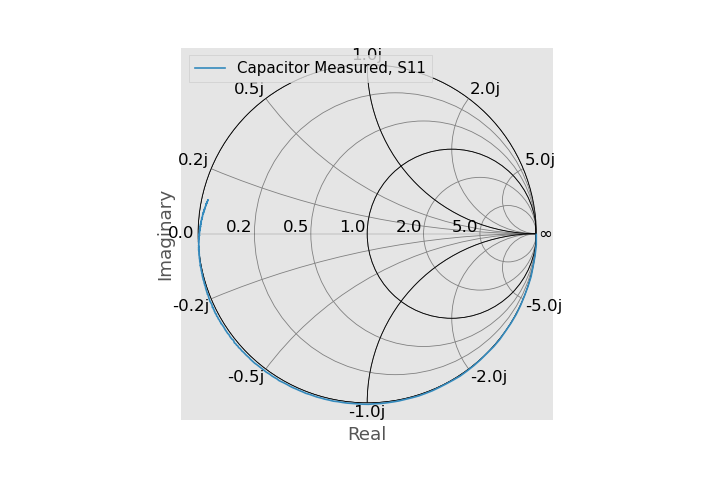
\includegraphics[width=.9\linewidth]{./pics/capacitor_meas_smith.png}
        \caption{S11 on Smith Chart}
    \end{subfigure}%
    \begin{subfigure}{0.5\linewidth}
        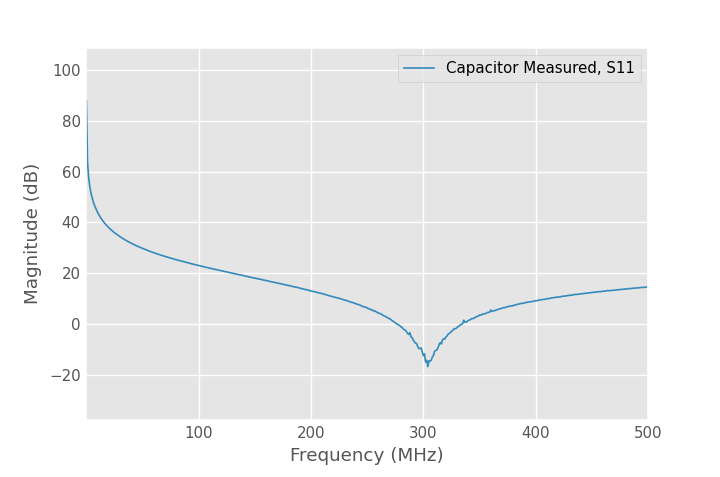
\includegraphics[width=.9\linewidth]{./pics/capacitor_meas_db.png}
        \caption{Magnitude of Impedance}
    \end{subfigure}

    \begin{subfigure}{\linewidth}
        \centering
        \begin{tabular}{ |c|c|c| }
            \hline
            Frequency (MHz) & S11         & Impedance (Ohm)
            \\\hline
            0.05            & 1.00-0.00j  & 1114.88-24861.18j
            \\\hline
            10.049          & 0.82-0.58j  & -0.17-157.00j
            \\\hline
            100.04          & -0.86-0.53j & -0.41-14.14j
            \\\hline
            305.0195        & -0.99+0.00j & 0.19+0.01j
            \\\hline
            500             & -0.94+0.20j & 0.98+5.25j
            \\\hline
        \end{tabular}
        \caption{S11 and Impedance at certain frequencies}
    \end{subfigure}

    \caption{S Parameter of Measured Capacitor}
    \label{fig:capacitor_meas}
\end{figure}

We measured the S-Parameters of the capacitor in the kit (item 7 in \Cref{fig:test_loads}), and the results are depicted in \Cref{fig:capacitor_meas}.

\begin{figure}
    \centering
    \begin{subfigure}{.5\linewidth}
        \centering
        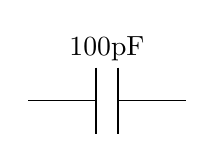
\begin{tikzpicture}
            \draw (0,0) to[C, label=100pF] ++(2,0);
        \end{tikzpicture}
        \caption{Ideal Capacitor Model}
        \label{fig:capacitor_c}
    \end{subfigure}%
    \begin{subfigure}{.5\linewidth}
        \centering
        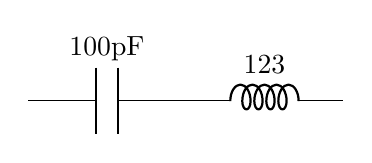
\begin{tikzpicture}
            \draw (0,0) to[C, label=100pF] ++(2,0)
            to[L, label=123] ++(2, 0);
        \end{tikzpicture}
        \caption{Capacitor with Series Inductance}
        \label{fig:capacitor_cl}
    \end{subfigure}%
    \caption{Electric Models of Real Life Capacitor}
\end{figure}

\begin{figure}
    \centering
    \begin{subfigure}{0.5\linewidth}
        \centering
        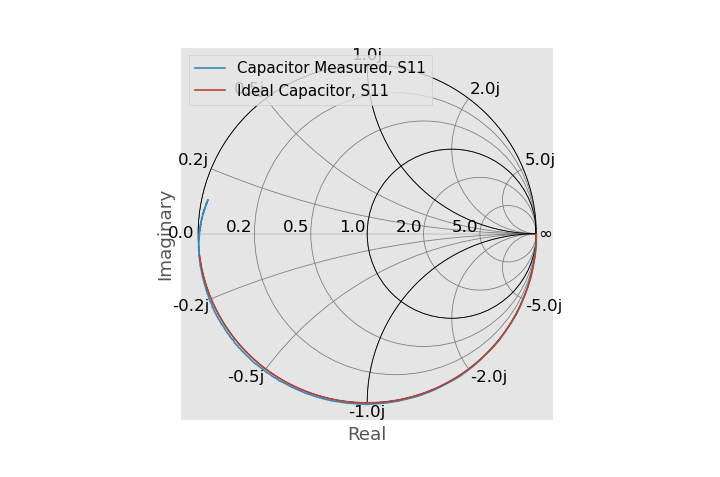
\includegraphics[width=\linewidth]{./pics/capacitor_models_smith.png}
        \caption{S11 of electric models of capacitor on Smith Chart}
    \end{subfigure}%
    \begin{subfigure}{0.5\linewidth}
        \centering
        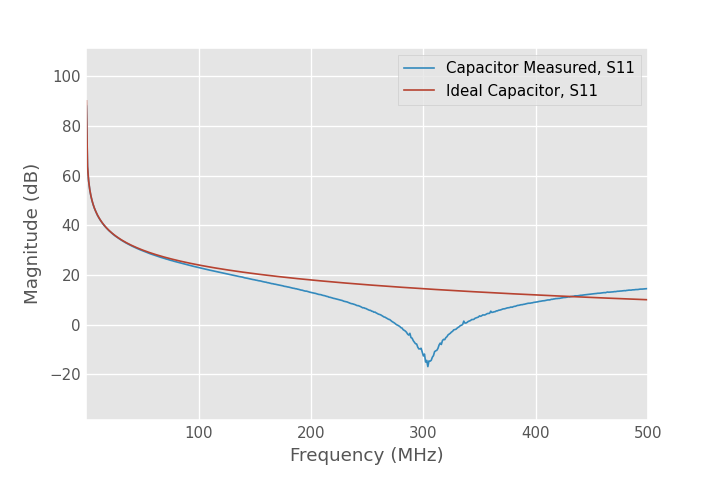
\includegraphics[width=\linewidth]{./pics/capacitor_models_db.png}
        \caption{Magnitude of Impedance of electric models of capacitor}
    \end{subfigure}
    \caption{Electric Characteristics of real capacitor compared with various models}
    \label{fig:capacitor_compare}
\end{figure}
\subsubsection{Ideal Capacitor Model}

Using the impendance at 10MHz, we see that the capacitance is roughly
$$\frac{1}{2\pi\cdot 10MHz \cdot 157 \Omega} \approx 100pF .$$
So our first model of the element would just be an ideal capacitor of $100pF$ (\Cref{fig:capacitor_c}).

However, immediately we see that the ideal capacitor does not fully characterize the real capacitor: in the Smith chart, S11 crosses the real axis and goes into the upper half of the unit circle, and in the impedance magnitude plot, the impedance has a minimum at around 300MHz.
(\Cref{fig:capacitor_compare})

\subsubsection{Parasitic Inductance}
Since the measured impedance of the capacitor goes up beyond 300MHz, this indicates the existance of some parasitic inductance.
Since parasitic inductance is often introduced by the magnetic field caused by conductors, we choose to model it as \textbf{series parasitic inductance} (\Cref{fig:capacitor_cl}).

The minimum impedance occurs at roughly 305MHz (which corresponds to S11 crossing the real axis).
This indicates that the 305MHz is the resonance frequency of the LC circuit.
So the series inductance can be calculated as
\[
    L = \frac{1}{(2\pi f)^2 C}
    = \frac{1}{(2\pi 305MHz)^2 \cdot 100pF}
    \approx
    2.7nH.
\]

\subsection{Inductor}

\end{document}